\documentclass[11pt,a4paper]{article}

\def\nyear {2025}
\def\nterm {Winter}
\def\nlecturer {}
\def\ncourse {Complex Analysis}

\makeatletter

% packages
\usepackage{amssymb,amsfonts,amsmath,calc,tikz,pgfplots,geometry,mathtools}
\usepackage{color}   % May be necessary if you want to color links
\usepackage[hidelinks]{hyperref}
\usepackage{forest}
\usepackage{commath}
\usepackage{amsthm}
\usepackage{fancyhdr}
\usepackage{bm}
\usepackage{witharrows}
\usepackage{bookmark}
\usepackage{tikz-cd}
\usepackage{bbm}
\usepackage{textcomp}
\usepackage{gensymb}
\usepackage{cleveref}

% tikz libraries
\usetikzlibrary{positioning}
\usetikzlibrary{matrix}
\usetikzlibrary{arrows}
\usetikzlibrary{arrows.meta}
\usetikzlibrary{decorations.markings}

% Page style setup
\pagestyle{fancy}
\geometry{margin=1in}
\pgfplotsset{compat=1.18}
\setlength{\headheight}{14.6pt}
\addtolength{\topmargin}{-1.6pt}
\hypersetup{
    colorlinks=false,
    linktoc=section,
    linkcolor=black,
}

%% maketitle setup
\ifx \nauthor\undefined
  \def\nauthor{yehelip}
\else
\fi

\ifx \ncoursehead \undefined
\def\ncoursehead{\ncourse}
\fi

\lhead{\emph{\nouppercase{\leftmark}}}
\ifx \nextra \undefined
  \rhead{
    \ifnum\thepage=1
    \else
      \ncoursehead
    \fi}
\else
  \rhead{
    \ifnum\thepage=1
    \else
      \ncoursehead \ (\nextra)
    \fi}
\fi

\let\@real@maketitle\maketitle
\renewcommand{\maketitle}{\@real@maketitle\begin{center}
\begin{minipage}[c]{0.9\textwidth}\centering\footnotesize
These notes are not endorsed by the lecturers.
I have revised them outside lectures to incorporate supplementary explanations,
clarifications, and material for fun.
While I have strived for accuracy, any errors or misinterpretations 
are most likely mine.
\end{minipage}\end{center}}

% theorem environments
\theoremstyle{definition}
\newtheorem{definition}{Definition}[section]
\newtheorem{remark}{Remark}[section]
\newtheorem{example}{Example}[section]
\newtheorem{exercise}{Exercise}[section]
\newtheorem{paradox}{Paradox}[section]
\newtheorem*{solution}{Solution}
\theoremstyle{plain}
\newtheorem{theorem}{Theorem}[section]
\newtheorem{proposition}[theorem]{Proposition}
\newtheorem{lemma}[theorem]{Lemma}
\newtheorem{corollary}[theorem]{Corollary}

% tikz customization
\pgfarrowsdeclarecombine{twolatex'}{twolatex'}{latex'}{latex'}{latex'}{latex'}
\tikzset{->/.style = {decoration={markings,
                                  mark=at position 1
                                  with {\arrow[scale=2]{latex'}}},
                      postaction={decorate}}}
\tikzset{<-/.style = {decoration={markings,
                                  mark=at position 0 with {\arrowreversed[scale=2]{latex'}}},
                      postaction={decorate}}}
\tikzset{<->/.style = {decoration={markings,
                                   mark=at position 0 with {\arrowreversed[scale=2]{latex'}},
                                   mark=at position 1 with {\arrow[scale=2]{latex'}}},
                       postaction={decorate}}}
\tikzset{->-/.style = {decoration={markings,
                                   mark=at position #1 with {\arrow[scale=2]{latex'}}},
                       postaction={decorate}}}
\tikzset{-<-/.style = {decoration={markings,
                                   mark=at position #1 with {\arrowreversed[scale=2]{latex'}}},
                       postaction={decorate}}}
\tikzset{->>/.style = {decoration={markings,
                                  mark=at position 1 with {\arrow[scale=2]{latex'}}},
                      postaction={decorate}}}
\tikzset{<<-/.style = {decoration={markings,
                                  mark=at position 0 with {\arrowreversed[scale=2]{twolatex'}}},
                      postaction={decorate}}}
\tikzset{<<->>/.style = {decoration={markings,
                                   mark=at position 0 with {\arrowreversed[scale=2]{twolatex'}},
                                   mark=at position 1 with {\arrow[scale=2]{twolatex'}}},
                       postaction={decorate}}}
\tikzset{->>-/.style = {decoration={markings,
                                   mark=at position #1 with {\arrow[scale=2]{twolatex'}}},
                       postaction={decorate}}}
\tikzset{-<<-/.style = {decoration={markings,
                                   mark=at position #1 with {\arrowreversed[scale=2]{twolatex'}}},
                       postaction={decorate}}}

\pgfarrowsdeclare{biggertip}{biggertip}{%
  \setlength{\arrowsize}{1pt}
  \addtolength{\arrowsize}{.1\pgflinewidth}
  \pgfarrowsrightextend{0}
  \pgfarrowsleftextend{-5\arrowsize}
}{%
  \setlength{\arrowsize}{1pt}
  \addtolength{\arrowsize}{.1\pgflinewidth}
  \pgfpathmoveto{\pgfpoint{-5\arrowsize}{4\arrowsize}}
  \pgfpathlineto{\pgfpointorigin}
  \pgfpathlineto{\pgfpoint{-5\arrowsize}{-4\arrowsize}}
  \pgfusepathqstroke
}
\tikzset{
	EdgeStyle/.style = {>=biggertip}
}

\tikzset{circ/.style = {fill, circle, inner sep = 0, minimum size = 3}}
\tikzset{scirc/.style = {fill, circle, inner sep = 0, minimum size = 1.5}}
\tikzset{mstate/.style={circle, draw, black, text=black, minimum width=0.7cm}}

\tikzset{eqpic/.style={baseline={([yshift=-.5ex]current bounding box.center)}}}

\definecolor{mblue}{rgb}{0.2, 0.3, 0.8}
\definecolor{morange}{rgb}{1, 0.5, 0}
\definecolor{mgreen}{rgb}{0, 0.4, 0.2}
\definecolor{mred}{rgb}{0.5, 0, 0}

% algebra
\DeclareMathOperator{\lcm}{lcm}
\DeclareMathOperator{\Out}{Out}
\DeclareMathOperator{\Aut}{Aut}
\DeclareMathOperator{\End}{End}
\DeclareMathOperator{\Inn}{Inn}
\DeclareMathOperator{\Mat}{Mat}
\DeclareMathOperator{\std}{std}
\DeclareMathOperator{\sgn}{sgn}
\DeclareMathOperator{\id}{id}
\newcommand{\idealin}{\triangleleft}
\newcommand{\ip}[2]{\langle #1, #2 \rangle}
\newcommand{\bigslant}[2]
{{\raisebox{.2em}{$#1$}\left/\raisebox{-.2em}{$#2$}\right.}}

% analysis
\newcommand{\dx}{\dif x}
\newcommand{\dt}{\dif t}
\newcommand{\du}{\dif u}
\newcommand{\dv}{\dif v}
\DeclareMathOperator{\im}{im}
\DeclareMathOperator{\cis}{cis}
\DeclareMathOperator{\Int}{Int}
\DeclareMathOperator{\diam}{diam}
\DeclareMathOperator{\supp}{supp}
\DeclareMathOperator{\Vol}{Vol} % Volume

% logic
\DeclareMathOperator{\MOD}{MOD}
\DeclareMathOperator{\Theory}{Theory}


% nice
\newcommand{\half}{\frac{1}{2}}
\newcommand{\pair}{\del}
\newcommand{\taking}[1]{\xrightarrow{#1}}
\newcommand{\inv}{^{-1}}
\newcommand{\ot}{\leftarrow}
\newcommand{\ninfty}{-\infty}
\newcommand{\floor}[1]{\left\lfloor #1 \right\rfloor}
\newcommand{\ceil}[1]{\left\lceil #1 \right\rceil}

% probability
\newcommand{\Prob}{\mathbf{P}}
\renewcommand{\vec}[1]{\boldsymbol{\mathbf{#1}}}
\DeclareMathOperator{\Bin}{Bin}
\DeclareMathOperator{\Geo}{Geo}
\DeclareMathOperator{\Poi}{Poi}
\DeclareMathOperator{\Exp}{Exp}
\DeclareMathOperator{\Var}{Var} % Variance
\DeclareMathOperator{\Cov}{Cov}

% special letters
\newcommand{\N}{\mathbb{N}}
\newcommand{\Z}{\mathbb{Z}}
\newcommand{\Q}{\mathbb{Q}}
\newcommand{\R}{\mathbb{R}}
\newcommand{\C}{\mathbb{C}}
\newcommand{\F}{\mathbb{F}}
\newcommand{\E}{\mathbb{E}}
\newcommand{\ps}{\mathcal{P}}
\newcommand{\M}{\mathcal{M}}
\renewcommand{\L}{\mathcal{L}}
\newcommand{\Omicron}{O}
\newcommand{\powerset}{\mathcal{P}}

% text
\newcommand{\st}{\text{ s.t. }}
\newcommand{\tand}{\quad \text{and} \quad}
\newcommand{\tor}{\quad \text{or} \quad}
\newcommand{\stand}{\text{ and }}
\newcommand{\stor}{\text{ or }}
\renewcommand{\tt}[1]{\textnormal{\textbf{(#1).}}} %tt=theorem title GET RID OF

% title format
\title{\textbf{\ncourse}}
\author{Based on lectures by \nlecturer \\\small Notes taken by \nauthor}
\date{\nterm\ \nyear}
\makeatother


\newcommand{\powerseries}{\sum_{n=0}^{\infty} a_n (z - z_0)^n}
\newcommand{\length}{\mathrm{length}}

\begin{document}
\maketitle

% Insert cool image here

\newpage
\tableofcontents
\newpage

\section{Introduction}

\subsection{Complex numbers and the complex plane}

\subsubsection{Preliminaries}

\begin{definition}[Complex number]
  A complex number is an expression of the form $x + yi$ such that
  $x,y \in \R$ and $i$ is a `imaginary number' not in $\R$.
  We denote
  \[
      \Re(z) := x \tand \Im(z) := y.
  \]
  If $\Im(z) = 0$ then $z$ is said to be a real number, and if
  $\Re(z) = 0$ then it is said to be purely imaginary.
\end{definition}

The set of all complex numbers is denoted as $\C$ and it can be made into
a field with the following operations.
\[
  z_1 + z_2 = (x_1 + x_2) + (y_1 + y_2) i \tand
  z_1 z_2 = (x_1 x_2 - y_1 y_2) + (x_1 y_2 + y_1 x_2) i.
\]
The field $\C$ is called the complex plane.

Note that $i^2 = -1$.
Also note that $T(x + y i) = (x, y)$ is a bijection between $\C$ and $\R$ and
moreover, we have that $T$ is additive.
That is
\[
  T(z_1 + z_2) = T(z_1) + T(z_2)
\]
which gives complex addition a geometric meaning.

\begin{center}
  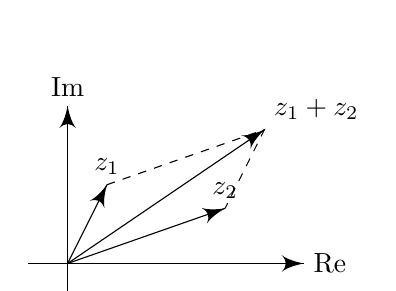
\begin{tikzpicture}
    \draw [->] (-0.5, 0) -- (3, 0) node [right] {Re};
    \draw [->] (0, -0.5) -- (0, 2) node [above] {Im};
    \draw [->] (0, 0) -- (.5, 1) node [above] {$z_1$};
    \draw [->] (0, 0) -- (2, .7) node [above] {$z_2$};
    \draw [->] (0, 0) -- (2.5, 1.7) node [anchor=south west] {$z_1 + z_2$};
    \draw [dashed] (.5, 1) -- (2.5, 1.7) -- (2, .7);
  \end{tikzpicture}
\end{center}

The absolute value of a complex number $x + y i = z \in \C$ is defined by
\[
  |z| = \sqrt{x^2 + y^2}.
\]
Note that $|z| = \norm{(x,y)}= \norm{T(z)}$ where $\norm{\cdot}$ is the standard
Euclidean norm on $\R^2$.

This implies that $|z - w|$ should be considered the distance between natural
numbers $z$, $w$.
Because we have that $|z| = \norm{T(z)}$ we also have that the triangle
inequality holds:
\[
  |z + w| \le |z| + |w| \text{ for all } z,w \in \C.
\]

\begin{definition}[Complex conjugate]
  The complex conjugate of $x + y i = z \in C$ is the complex number
  $x - y i$. The complex conjugate of $z$ is denoted $\bar{z}$.
\end{definition}

\begin{center}
  \begin{tikzpicture}
    \draw [->] (-0.5, 0) -- (3, 0) node [right] {Re};
    \draw [->] (0, -1) -- (0, 2) node [above] {Im};
    \draw [->] (0, 0) -- (2, .7) node [above] {$z_2$};
    \draw [->] (0, 0) -- (2, -.7) node [above] {$\bar z_2$};
  \end{tikzpicture}
\end{center}

It is easy to verify that
\[
  \Re(z) = \frac{z + \bar{z}}{2} \tand 
  \Re(z) = \frac{z - \bar{z}}{2 i} \tand
  |z|^2 = z \bar{z}.
\]

Given $\theta$ we can denote $e^{i \theta} = \cos \theta + i \sin \theta$,
and then describe any complex number $z \in \C$ as $r e^{i \theta}$
for some $\theta \in [0, 2\pi)$ and $r > 0$.
We get that $|z| = |r e^{i \theta}| = r$.
We also have that $\theta$ describes the angle of $z$ with the $x$-axis
and it is usually denoted $\theta = \arg(z)$.

\subsubsection{Convergence}

\begin{definition}[Convergence]
  We say that the sequence $\set{z_n}_{n \geq 1} \subset \C$ converges
  to some $z_0 \in \C$ if $|z - z_0| \taking{n \to \infty} 0$.
  In this case, we call $z_0$ the limit of the sequence of
  $\set{z_n}_{n \geq 1}$.
\end{definition}

\begin{remark}
  It is easy to verify that the limit is unique, and that
  $z_n \taking{n \to \infty} z$ if and only if
  $T(z_n) \taking{n \to \infty} T(z)$ in the Euclidean metric.
\end{remark}

\begin{definition}[Cauchy sequence]
  A sequence $\set{z_n}_{n \geq 1}$ is said to be a Cauchy sequence if for
  all $\epsilon > 0$ there exists $N > 1$ such that for all $n,m > N$
  we have that $|z_n - z_m| < \epsilon$.
\end{definition}

\begin{proposition}
  The complex plane $\C$ is complete.
  That is, every Cauchy sequence converges in $\C$.
\end{proposition}
\begin{proof}
  The proof follows immediately from the known fact that $\R$ is complete
  and the previous remark.
\end{proof}

\subsubsection{Sets in the complex plane}

\begin{definition}[Open disc]
  For $z_0 \in \C$ and $r > 0$ we set
  \[
      D_r(z_0) := \set{z \in \C \colon |z - z_0| < r}.
  \]
  We call $D_r(z_0)$ the open disc at center $z_0$ with radius $r$.
\end{definition}


\begin{definition}[Closed disc]
  For $z_0 \in \C$ and $r > 0$ we set
  \[
      \overline D_r(z_0) := \set{z \in \C \colon |z - z_0| \le r}.
  \]
  We call $\overline D_r(z_0)$ the closed disc at center $z_0$ with
  radius $r$.
\end{definition}

\begin{definition}[Circle]
  For $z_0 \in \C$ and $r > 0$ we set
  \[
      C_r(z_0) := \set{z \in \C \colon |z - z_0| = r}.
  \]
  We call $C_r(z_0)$ the circle at center $z_0$ with radius $r$.
\end{definition}

\begin{definition}[Interior point]
  Given $\Omega \subset \C$, we say that $z \in \Omega$ is an interior
  point of $\Omega$ if exists $r > 0$ such that $D_r(z) \subset \Omega$.
\end{definition}

\begin{definition}[Interior of a set]
  Given $\Omega \subset \C$, we say that the interior of $\Omega$ is
  the collection of all interior points of $\Omega$.
  We denote the interior as $\Int(\Omega)$.
\end{definition}

\begin{definition}[Open set]
  Given $\Omega \subset \C$, we say that $\Omega$ is an open set if
  $\Int(\Omega) = \Omega$.
\end{definition}

\begin{definition}[Closed set]
  Given $\Omega \subset \C$, we say that $\Omega$ a closed set if
  $\Omega^c := \C \setminus \Omega$ is open.
\end{definition}

\begin{definition}[Limit point]
  Given $\Omega \subset \C$, we say that $z \in \Omega$ is an interior
  point of $\Omega$ if there exists a sequence $z_n$ such that
  $z_n \neq z$ for all $n > 1$ and $z_n \taking{n \to \infty} z$.
\end{definition}

\begin{proposition}
  Let $\Omega \subset \C$ be given.
  Then $\Omega$ is closed if and only if it contains
  all of its limit points.
\end{proposition}
\begin{proof}
  Clear.
\end{proof}

\begin{definition}[Closure]
  Let $\Omega \subset \C$ be given.
  The closure of $\Omega$, denoted $\overline \Omega$, is defined
  as
  \[
      \overline \Omega =
      \Omega \cup
      \set{z \in \C \mid \text{$x$ is a limit point of $\Omega$}}.
  \]
\end{definition}

\begin{remark}
  Note that $\Omega$ is closed if and only if $\overline \Omega = \Omega$.
\end{remark}

\begin{definition}[Boundary]
  The boundary of $\Omega \subset \C$ is denoted by $\partial \Omega$
  and defined by $\partial \Omega := \Omega \setminus \Int(\Omega)$.
\end{definition}

\begin{definition}[Diameter]
  Given $\Omega \subset \C$, we define the diameter of $\Omega$ as
  \[
      \diam(\Omega) := \sup\set{|z - w| \colon z,w \in \Omega}.
  \]
\end{definition}

\begin{definition}[Bounded set]
  Given $\Omega \subset \C$, we say that $\Omega$ is bounded if
  $\diam(\Omega) < \infty$.
\end{definition}

\begin{remark}
  It is clear that a set $\Omega \subset \C$ is bounded if and only if
  there exists $z_0 \in \C$ and $r > 0$ such that $\Omega \subset D_r(z_0)$.
\end{remark}

\begin{definition}[Compact set]
  A subset $\Omega$ of $\C$ is said to be compact if it is closed and 
  bounded.
\end{definition}

\begin{theorem}\tt{Bolzano--Weierstrass theorem}
  A subset $\Omega$ in $\C$ is compact if and only if every seqeuence
  $\set{z_n}_{n \geq 1}$ has a subsequence $\set{z_{n_k}}$ such that
  $z_{n_k} \taking{k \to \infty} z$ for some $z \in \C$.
\end{theorem}

\begin{theorem}\tt{Cantor's intersection lemma}
  Let $\Omega_1, \Omega_2, \dots$ be nonempty compact subsets of $\C$.
  Suppose that $\Omega_{n+1} \subset \Omega_n$ for all $n \geq 1$,
  and that $\diam(\Omega_n) \taking{n \to \infty} 0$.
  Then $\cap_{n \geq 1} \Omega_n = \set{z}$ for some $z \in \C$.
\end{theorem}
\begin{proof}
  Choose $z_n \in \Omega_n$ for all $n \geq 1$.
  Because $\diam \Omega \taking{n \to \infty} = 0$ we have that
  $\set{z_n}_{n \geq 1}$ is a Cauchy sequence and therefore it converges
  to some $z \in \C$. Because $\Omega_n$ is compact for every $n \geq 1$
  we get that $z \in \cap_{n \geq 1} \Omega_n$.
  This means that $\cap_{n \geq 1} \Omega_n \neq \emptyset$.

  Let $z,w \in \Omega$.
  Because $\diam \Omega \taking{n \to \infty} 0$ we have that
  $|z - w| \le 0$ and thus $z = w$ which implies that
  $\cap_{n \geq 1} \Omega_n = \set{z}$ which completes the proof.
\end{proof}

\begin{definition}[Connected open set]
  A nonempty open set $\Omega \subset \C$ is said to be connected if it does
  not contain disjoint nonempty open subsets $\Omega_1$, $\Omega_2$ such
  that $\Omega = \Omega_1 \cup \Omega_2$. A connected open set in 
  $\C$ will be called a region.
\end{definition}

\begin{definition}[Connected closed set]
  A nonempty open set $\Omega \subset \C$ is said to be connected if it does
  not contain disjoint nonempty closed subsets $\Omega_1$, $\Omega_2$ such
  that $\Omega = \Omega_1 \cup \Omega_2$.
\end{definition}

\begin{remark}
  It can be shown that $\Omega$ is connected if and only if for any
  $z, w \in \Omega$ there exists a curve $\gamma \colon [0,1] \to \Omega$
  such that $\gamma(0) = z$ and $\gamma(1)$.
  This implies that open and closed discs, as well as circles, are
  connected.
\end{remark}

\subsubsection{Continuous functions}

\begin{definition}[Continuous function]
  Let $\Omega$ be a nonempty subset of $\C$ and let 
  $f \colon \Omega \to \C$ be given.
  We say that $f$ is continuous at a point $z_0 \in \Omega$ 
  if for all $\epsilon > 0$ there exists $\delta > 0$ so
  that $|f(z) - f(z_0)| < \epsilon$ for all $z \in \Omega$ with 
  $|z - z_0| < \delta$.
  We say that $f$ is continuous on $\Omega$ if it is continuous at every 
  $z_0 \in \Omega$.
\end{definition}

\begin{remark}
  It is easy to verify that the functions $\Im$, $\Re$, $|\cdot|$, and
  $\theta \mapsto e^{i \theta}$ are all continuous.
\end{remark}

\begin{proposition}
  The composition of continuous functions is continuous.
\end{proposition}

\begin{definition}[Bounded function]
  Let $\Omega$ be a nonempty subset of $\C$ and let 
  $f \colon \Omega \to \C$ be given.
  We say that $f$ is bounded if there exists $M > 0$ so that 
  $|f(z)| < M$ for all $z \in \Omega$.
  We say that $f$ attains a maximum if there exists $z_M \in \Omega$
  such that $f(z) \le f(z_M)$ for all $z \in \Omega$.
  We define when $f$ attains a minimum similarly.
\end{definition}

\begin{proposition}
  Let $\Omega$ be a nonempty compact subset of $\C$, and let 
  $f \colon \Omega \to \C$ be continuous.
  Then $f$ is bounded, and it attains its maximum and minimum on $\Omega$.
\end{proposition}

\subsection{Holomorphic functions}

\begin{definition}[Holomorphic function]
  Let $\Omega$ be a nonempty open subset of $\C$ and let 
  $f \colon \Omega \to \C$ be given.
  We say that $f$ is holomorphic at a point $z \in \Omega$
  if the following limit exists
  \[
      f'(z) := \lim_{h \to 0} \frac{f(z + h) - f(z)}{h}.
  \]
  The number $f'(z)$ is called the derivative of $f$ at $z$.
  It is said that $f$ is holomorphic if it is holomorphic at every
  $z \in \Omega$.
  Given a closed subset $C \subset \Omega$, we say that $f$ is holomorphic
  on $C$ if there exists $C \subset \Omega' \subset \Omega$ so that
  $\Omega'$ is open and $f$ is holomorphic on $\Omega'$.
\end{definition}

\begin{definition}[Entire function]
  We say that $f \colon \C \to \C$ is entire if it is holomorphic on $\C$.
\end{definition}

\begin{remark}
  Note that $h$ is a complex number and can approach $0$ from any direction.
\end{remark}

\begin{remark}
  It is also useful to notice that $f \colon \Omega \to \C$ is holomorphic
  at $z \in \Omega$ if and only if there exist $a \in \C$, $r > 0$ with
  $D_r(z) \subset \Omega$, and a function $\psi \colon D_r(0) \to \C$ with
  $\lim_{h \to 0} \psi(h) = 0$, so that
  \[
    f(z + h) = f(z) + ah + h \psi(h) \text{ for all } h \in D_r(0).
  \]
  From this formulation is it clear that $f$ is continuous at $z$ whenever
  $f$ is holomorphic at $z$.
\end{remark}

\begin{example}
  It follows directly from the definition that the function $1/z$ is holomorphic
  on $\C \setminus \set{0}$ with $f'(z) = -1/z^2$. For all $0 \neq z \in \C$
  we have
  \[
    \lim_{h \to 0} \frac{f(z + h) - f(z)}{h} =
    \lim_{h \to 0} \frac{1}{h} \del{\frac{1}{z + h} - \frac{1}{z}} =
    \lim_{h \to 0} \frac{-1}{z (z + h)} =
    \frac{-1}{z^2}.
  \]
\end{example}

\begin{example}
  The function $f(z) = \bar z$ is not holomorphic. For any $z \in \C$ and
  $r \in \R$ we have that
  \[
    \frac{f(z + t) - f(z)}{t} = 1 \tand
    \frac{f(z + t i) - f(z)}{t i} = -1
  \]
\end{example}

\begin{proposition}
  \label{prop:holo-is-linear}
  Let $\Omega \subset \C$ be open and let $f,g \colon \Omega \to \C$ be
  holomorphic at $z \in \Omega$. Then
  \begin{enumerate}
    \item[(1)] $f + g$ is holomorphic at $z$ with $(f + g)'(z) = f'(z) + g'(z)$.
    \item[(2)] $f g$ is holomorphic at $z$ with $(f g)'(z) = 
      f'(z)g(z) + f(z)g'(z)$.
  \end{enumerate}
\end{proposition}

\begin{proof}
  We will only prove $(2)$ because the proof of $(1)$ is much simpler.
  Because $f$ and $g$ are holomorphic at $z$, they are also continuous
  there. Thus,
  \begin{align*}
    \lim_{h \to 0} \frac{(f g)(z + h) - (f g)(z)}{h} &=
    \lim_{h \to 0} \del{\frac{f(z + h) - f(z)}{h} g(z + h) + 
  f(z) \frac{g(z + h) - g(z)}{h}} \\ &=
    f'(z)g(z) + f(z)g'(z),
  \end{align*}
  which completes the proof.
\end{proof}

\begin{corollary}
  It's quite easy to prove that constant function of the form $f(z) = c$
  for some $c \in \C$ and $f(z) = z$ are holomorphic.
  It follows immediately from \Cref{prop:holo-is-linear} that all polynomials,
  functions of the form $p(z) = \sum_{k=0}^{n} a_k z^k$ are entire, with
  $p'(z) = \sum_{k=1}^{n} k a_k z^{k-1}$ for all $z \in \C$.
\end{corollary}

\begin{proposition}
  A composition of holomorphic functions at $z$ is holomorphic at $z$, with
  $(g \circ f)'(z) = g'(f(z)) f'(z)$.
\end{proposition}

\begin{corollary}
  Let $\Omega \subset \C$ be open and let $f,g \colon \Omega \to \C$ be
  holomorphic at $z \in \Omega$.
  Suppose also that $g(z) \neq 0$.
  Then $f/g$ is holomorphic at $z$ with
  \[
    (f/g)'(z) = \frac{f'(z)g(z) + f(z)g'(z)}{g(z)^2}.
  \]
\end{corollary}
\begin{proof}
  Let $h \colon \C \setminus \set{0} \to \C$ be with $h(z) = 1/z$.
  We now have that
  \begin{align*}
    (f/g)'(z) &=
    (f \cdot (h \circ g))'(z) =
    f'(z)(h \circ g)(z) + f(z)(h \circ g)'(z) \\ &=
    f'(z)/g(z) + f(z)h'(g(z))g'(z) =
    f'(z)/g(z) - f(z)g(z)^{-2}g'(z).
  \end{align*}
\end{proof}

Recall that $T \colon \C \to \R^2$ is the operator $T(x + y i) = (x,y)$.

\begin{proposition}
  \label{prop:pd}
  Let $\Omega \subset \C$ be open, let $f \colon \Omega \to \C$, let 
  $u,v \colon T(\Omega) \to \R$ be with $f(x + y i) = u(x,y) + i v(x,y)$
  for $x + i y \in \Omega$, and let $F \colon T(\Omega) \to \R^2$ be with
  $F(x,y) = (u(x,y), v(x,y))$ for $(x,y) \in T(\Omega)$.
  Fix $x_0 + i y_0 = z_0 \in \Omega$,
  write $p = (x_0, y_0)$, and suppose that $f$ is holomorphic at $z_0$.
  Then,
  \begin{enumerate}
    \item[(1)] the partial derivatives of $u$ and $v$ exist at $p$, and
      \[
        f'(z_0) =
        \pd{u}{x}(p) + i \pd{v}{x}(p) =
        \pd{v}{y}(p) - i \pd{u}{y}(p);
      \]
    \item[(2)] The Cauchy--Riemann equations are satisfied:
      \[
        \pd{u}{x}(p) = \pd{v}{y}(p) \stand
        \pd{u}{y}(p) = -\pd{v}{x}(p).
      \]
    \item[(3)] $F$ is differentiable at $p$ with,
      \[
        dF_p =
        \begin{pmatrix}
          \pd{u}{x}(p) & - \pd{v}{x}(p) \\
          \pd{v}{x}(p) & \pd{u}{x}(p) 
        \end{pmatrix} =
        \begin{pmatrix}
          \pd{v}{y}(p) & \pd{u}{y}(p) \\
          - \pd{u}{y}(p) & \pd{v}{y}(p) 
        \end{pmatrix}.
      \]
  \end{enumerate}
\end{proposition}

\begin{remark}
  Note that $u = \Re \circ f \circ T^{-1}$, $v = \Im \circ f \circ T^{-1}$
  and $F = T \circ f \circ T^{-1}$.
  Thus, $F$ is the map corresponding to $f$ under the identification of $\C$ 
  with $\R^2$ via $T$.
\end{remark}

\begin{remark}
  Note that from $(3)$ we have
  \[
    \det(dF_p) = \del{\pd{u}{x}(p)}^2 + \del{\pd{v}{x}(p)}^2.
  \]
  From this and from $(1)$, it follows that $\det(dF_p) > 0$ whenever
  $f'(z_0) \neq 0$.
  Moreover, we have that $\sqrt{\det(dF_p)} \cdot dF_p$ is an orthogonal
  matrix.
\end{remark}

We now prove \Cref{prop:pd}.

\begin{proof} \phantom{}
\begin{enumerate}
  \item[(1)] We can first let $t \to 0$ in $\R$ and see that
  \begin{align*}
    f'(z_0) &= \lim_{t \to 0} \frac{f(z + t) - f(z)}{h} \\
            &= \lim_{t \to 0} \frac{u(x_0 + t, y_0) - u(x_0,y_0) + 
            i v(x_0 + t, y_0) - i v(x_0,y_0)}{t} \\
            &= \diffp{u}{x}(p) + i \diffp{v}{x}(p).
  \end{align*}
  Similarly,
  \begin{align*}
    f'(z_0) &= \lim_{t \to 0} \frac{f(z + i t) - f(z)}{h} \\
            &= \lim_{t \to 0} \frac{u(x_0, y_0 + t) - u(x_0,y_0) + 
            i v(x_0, y_0 + t) - i v(x_0,y_0)}{t} \\
            &= \diffp{v}{y}(p) - i \diffp{u}{y}(p)
  \end{align*}
  which completes the proof of $(1)$.
  From the equation
  \[
     \pd{u}{x}(p) + i \pd{v}{x}(p) = \pd{v}{y}(p) - i \pd{u}{y}(p)
  \]
  \item[(2)] This is an immediate result of $(1)$.
  \item[(3)]
\end{enumerate}
\end{proof}

The following proposition is a kind of converse to the previous proposition.

\begin{proposition}
  Let $\Omega \subset \C$ be open, let $f \colon \Omega \to \C$,
  and let $u$ and $v$ be as in \Cref{prop:pd}.
  Fix $x_0 + i y_0 = z_0 \in \Omega$, write $p := (x_0,y_0)$,
  ans suppose that $u$ and $v$ are differentiable at $p$,
  that is $\pd{u}{x}(p) = \pd{v}{y}(p)$ and $\pd{u}{y}(p) = - \pd{v}{x}(p)$.
  Then $f$ is holomorphic at $z_0$.
\end{proposition}
\begin{proof}
  To be added.
\end{proof}

\subsection{Power series}

\begin{definition}[Power series]
  A power series centered at $z_0 \in \C$ is an expression of the
  form $\sum_{0}^{\infty} a_n (z - z_0)^n$,
  where $\set{a_n}_{n \geq 0} \subset \C$.
  Given $z \in \C$, we say that the power series converges at $z$ if
  the limit $\lim_{N \to \infty} \sum_{n=0}^{N} a_n (z - z_0)^n$ exists
  in $\C$.
  If this limit does not exist, we say that the series diverges at $z$.
\end{definition}

\begin{definition}[Absolute convergence]
  Given a power series $\sum_{n=0}^{\infty} a_n (z - z_0)$,
  we say that it converges absolutely at $z \in \C$ if
  $\sum_{n=0}^{\infty} \abs{a_n} \cdot \abs{(z - z_0)} < \infty$.
\end{definition}

\begin{proposition}
  If a power series converges absolutely at $z$ then it also converges at $z$.
  This follows from the completeness of $\C$.
\end{proposition}

In the following proposition we use the convention that $\frac{1}{0} = \infty$
and $\frac{1}{\infty} = 0$.

\begin{proposition}[Hadamard's theorem]
  \label{thm:hadamard}
  Let $\powerseries$ be a power series, and let $0 \le \R \le \infty$
  be given by
  \[
    \frac{1}{R} = \limsup_{n \to \infty} \abs{a_n}^{\frac 1n}.
  \]
  Then for $z \in \C$ the series converges absolutely if $|z - z_0| < R$,
  and the series diverges if $|z - z_0| > R$.
\end{proposition}

\begin{remark}
  The number $R$ is called the radius of convergence of the power series,
  and the region $\set{z \in \C \colon |z - z_0| < R}$ is called the disc
  of convergence.
\end{remark}

We now proceed to prove \Cref{thm:hadamard}

\begin{proof}
  Set $L := 1/R$.
  Suppose first that $0 < R \le \infty$, so that $0 \le L < \infty$.
  Let $z \in \C$ be such that $|z - z_0| < R$, then there exists
  $L < M < \infty$ so that $M |z - z_0| < 1$.
  By the definition of $L$ (the limsup) there exists $N \geq 1$ so that
  $|a_n|^{\frac 1n} < M$ forall $n > N$. Thus
  \begin{align*}
    \sum_{n=0}^{\infty} |a_n| \cdot |z - z_0|^n &=
    \sum_{n=0}^{N-1} |a_n| \cdot |z - z_0|^n +
    \sum_{n=N}^{\infty} \del{|a_n|^{\frac 1n} \cdot |z - z_0|}^n \\ &\le
    \sum_{n=0}^{N-1} |a_n| \cdot |z - z_0|^n +
    \sum_{n=N}^{\infty} \del{M |z - z_0|}^n <
    \infty.
  \end{align*}
  Suppose next that $0 \le R < \infty$, so that $0 < L \infty$.
  Let $z \in \C$ be such that $|z - z_0| > R$, then similarly there
  exists $0 < M < L$ so that $M |z - z_0| > 1$.
  Then, for every $N \geq 1$ there exists $n \geq N$ so that 
  $|a_n|^{\frac 1n} > M$.
  For such $n$ we have
  \begin{align*}
    \abs{\sum_{k=0}^{n} a_k(z-z_0)^k - \sum_{k=0}^{n-1} a_k(z-z_0)^k} &=
    |a_n| \cdot |z - z_0|^n \\ &=
    \del{|a_n|^{\frac 1n} \cdot |z - z_0|}^n >
    \del{M |z - z_0|}^n > 1,
  \end{align*}
  which shows that the partial sums do not form a Cauchy sequence.
  Thus the series diverges at $z$, which completes the proof.
\end{proof}

\begin{example}
  Considert the power series $e^z := \sum_{n=0}^{\infty} \frac{z^n}{n!}$.
  Because we have
  \[
    \sqrt[n]{(2n)!} \geq \sqrt[n]{n^n} = n
  \]
  we also have for every $n \geq 1$,
  \[
    \del{\frac{1}{(2n)!}}^{\frac{1}{2n}} \le \frac{1}{n^{\half}}
    \tand
    \del{\frac{1}{(2n+1)!}}^{\frac{1}{2n+1}} \le \frac{1}{n^{\half}}.
  \]
  Since $n^{-\half} \taking{n \to \infty} = 0$ we get that the radius of
  convergence is $\infty$ for the series.
  The map $z \mapsto e^z$ is called the exponantial function.
  We also have that
  \begin{align*}
    e^z e^w =
    \del{\sum_{n=0}^{\infty} \frac{z^n}{n!}} +
    \del{\sum_{n=0}^{\infty} \frac{w^n}{n!}} =
    \sum_{n=0}^{\infty}
    \frac{1}{n!} \sum_{k=0}^{n} \frac{n!}{k!(n-k)!} z^k w^{n-k} =
    \sum_{n=0}^{\infty} \frac{(z+w)^n}{n!} =
    e^{z + w}.
  \end{align*}
\end{example}

\begin{example}
  Consider the power series $f(z) := \sum_{n=0}^{\infty} z^n$.
  Since $1^{\frac 1n} = 1$ we get that the radius of convergence in
  this case is $1$.
  Thus $f$ defined a function from $D_1(0)$ to $\C$.
  Moreover, since we have
  \[
    (1 - z) \sum_{n=0}^{N} z^n = 1 - z^{N + 1},
  \]
  we get for $z \in D_1(0)$ that
  \[
    f(z) =
    \lim_{N \to \infty} \sum_{n=0}^{N} z^n =
    \lim_{N \to \infty} \frac{1 - z^{N + 1}}{1 - z} =
    \frac{1}{1 - z}.
  \]
\end{example}

\begin{proposition}
  \label{prop:holo-on-disc}
  Let $f(z) := \sum_{n=0}^{\infty} a_n (z - z_0)^n$ be a power series,
  and let $R$ be the radius of convergence of $f$. Then,
  \begin{enumerate}
    \item[(1)] $R$ is also the radius of convergence of
      $\sum_{n=0}^{\infty} n a_n (z - z_0)^{n - 1}$;
    \item[(2)] suppose $R > 0$, then $f$ is holomorphic in its disc of
      convergence with
      \[
        f'(z) = \sum_{n=1}^{\infty} n a_n (z - z_0)^{n - 1}.
      \]
  \end{enumerate}
\end{proposition}
\begin{proof}
\begin{enumerate} \phantom{}
  \item[(1)] Since $n^{1/n} \taking{n \to \infty} 1$ and
    $\frac{n-1}{n} \taking{n \to \infty} 1$, we have
    \[
      \frac{1}{R} =
      \limsup_{n \to \infty} |a_n|^{\frac{1}{n}} =
      \limsup_{n \to \infty} |n a_n|^{\frac{1}{n - 1}}
    \]
    which gives the first part of the proposition.
  \item[(2)] By the chain rule, the derivative of $f(z)$ wouldn't change
    for any $z_0 \in \C$ so we may choose $z_0 = 0$ and then
    $f(z) = \sum_{n=0}^{\infty} a_n z^n$.
    Suppose $R > 0$, let $0 < r < R$, fix $w \in D_r(0)$, and define
    \[
      g(z) := \sum_{n=1}^{\infty} n a_n (z - z_0)^{n - 1}.
    \]
    Since
    \[
      \sum_{n=1}^{\infty} n |a_n| r^{n - 1} \le
      \sum_{n=1}^{\infty} n |a_n| |z|^{n - 1} < \infty
    \]
    there exists $N \geq 1$ so that
    \[
      \sum_{n=N+1}^{\infty} n |a_n| r^{n - 1} < \frac{\epsilon}{3}.
    \]
    For $z \in D_r(0)$ set
    \[
      S(z) = \sum_{n=0}^{N} a_n z^n \stand
      E(z) = \sum_{n=N+1}^{\infty} a_n z^n.
    \]
    Since $w \in D_r(0)$ and $S$ is holomorphic at $w$ 
    (since it is a polynomial), there exists $\delta > 0$ so that
    $D_{\delta}(w) \subset D_r(0)$ and
    \begin{multline*}
      \left|
      \frac{f(w + h) - f(w)}{h} - g(w)
      \right| \le
      \left|
      \frac{S(w + h) - S(w)}{h} - S'(w)
      \right| +
      \left| S'(w) - g(w) \right| \\ +
      \left|
      \frac{E(w + h) - E(w)}{h}
      \right|.
    \end{multline*}
    Recall that
    \[
      S'(w) = \sum_{n=1}^{N} n a_n z^{n - 1}.
    \]
    Since $w \in B_r(0)$ we get
    \[
      \abs{S'(w) - g(w)} =
      \abs{\sum_{n=N+1}^{\infty} n a_n w^{n - 1}} \le
      \abs{\sum_{n=N+1}^{\infty} n |a_n| r^{n - 1}} <
      \frac{\epsilon}{3}.
    \]
    Notice that for each $n \geq 1$ and $a,b \in \C$,
    \[
      a^n - b^n =
      (a - b)(a^{n - 1} + a^{n - 2} b + \cdots + a b^{n-2} + b^{n-1}) =
      (a - b) \sum_{k=0}^{n-1} a^{n-k-1} b^{k}.
    \]
    Using this fact, and since $w,w+h \in D_r(0)$,
    \[
      \abs{(w + h)^n - w^n} =
      \abs{h \sum_{k=0}^{n-1} (w + h)^{n-k-1} w^{k}} \le
      |h| n r^{n-1}.
    \]
    We now have that
    \begin{align*}
      \abs{\frac{E(w + h) - E(w)}{h}} 
        &= \frac{1}{|h|} \abs{\sum_{n=N+1}^{\infty} a_n((w+h)^{n}-w^n)} \\
        &= \frac{1}{|h|} \sum_{n=N+1}^{\infty} |a_n| \cdot |(w+h)^{n}-w^n| \\
        &= \sum_{n=N+1}^{\infty} |a_n| n r^{n-1} < \frac{\epsilon}{3}.
    \end{align*}
    It now follows that
    \[
      \left|
      \frac{f(w + h) - f(w)}{h} - g(w)
      \right| < \epsilon \text{ for } 0 \neq h \in D_{\delta}(0).
    \]
    This shows that $f$ is holomorphic at $w$ with $f'(w) = g(w)$, which
    completes the proof.
\end{enumerate}
\end{proof}

\begin{corollary}
  A power series is infinitely complex differentiable in its disc of
  convergence, and the higher derivatives are also power series obtained 
  by termwise differentiation.
\end{corollary}

\begin{example}
  The function $e^z$ is entire with
  \[
    (e^z)' = \sum_{n=1}^{\infty} n \frac{z^{n-1}}{n!} = e^z
    \text{ for all } z \in \C.
  \]
\end{example}

\begin{example}
  The standard trigonometric functions are given by
  \[
    \cos z := \sum_{n=0}^{\infty} (-1)^n \frac{z^{2n}}{(2n)!} \stand
    \sin z := \sum_{n=0}^{\infty} (-1)^n \frac{z^{2n+1}}{(2n+1)!}.
  \]
  It is easy to verify that in both cases the radius of convergence
  is $\infty$.
  We also see that
  \[
    (\cos z)' = \sum_{n=1}^{\infty} (-1)^n \frac{z^{2n-1}}{(2n-1)!} = - \sin z
  \]
  and
  \[
    (\sin z)' = \sum_{n=0}^{\infty} (-1)^n \frac{z^{2n}}{(2n)!} = \cos z.
  \]
  From these equalities it is easy to check that $\sin z$ and $\cos z$ agree
  with their respective real versions.
  Moreover, a simple calculation gives the identities
  \[
    \cos z = \frac{e^{iz} + e^{-iz}}{2} \stand
    \sin z = \frac{e^{iz} - e^{-iz}}{2 i},
  \]
  which are called Euler formulas.
  By adding these identites we get
  \[
    e^{iz} = \cos z + i \sin z.
  \]
  It follows that for all $x,y \in \R$ we have
  \[
    e^{x + y i} = e^x e^{y i} = e^x (\cos y + i \sin y).
  \]
\end{example}

\begin{definition}[Analytic function]
  Let $\Omega \subset \C$ be open.
  A function $f \colon \Omega \to \C$ is said to be analytic at
  $z_0 \in \Omega$ if there exists a power series $\powerseries$,
  with radius of convergence $R > 0$, such that for some $0 < r < R$
  with $D_r(z_0) \subset \Omega$ we have
  \[
    f(z) = \powerseries \text{ for } z \in D_r(z_0).
  \]
  If $f$ has a power series expansion at every point in $\Omega$,
  we say that $f$ is analytic on $\Omega$.
\end{definition}

\begin{remark}
  From \Cref{prop:holo-on-disc} we get that an analytic function on $\Omega$
  is also holomorphic there. 
  A deep theorem theorem we shall prove later is that every holomorphic 
  function is analytic.
  This is why the terms holomorphic and analytic are often used interchangeably.
\end{remark}

\subsection{Integration along paths}
\begin{definition}[Path]
  A path (in $\C$) is a continuous function $\gamma \colon [a,b] \to \C$,
  where $a,b \in \R$ with $a < b$.
\end{definition}
\begin{definition}[Closed path]
  A closed path is a path such that $\gamma(a) = \gamma(b)$.
\end{definition}
\begin{definition}[Simple path]
  A path is called simple if $\gamma$ is injective, unless the path is closed,
  in which case we only require $\gamma\vert_{(a,b)}$ to be injective.
\end{definition}
\begin{remark}
  We sgakk write $\gamma^*$ for the image of $\gamma$, i.e.\
  $\gamma^* := \gamma([a,b])$.
  Note that $\gamma^*$ is a compact subset of $\C$.
\end{remark}

\begin{definition}[Differentiable path]
  Let $\gamma \colon [a, b] \to \C$ be a path.
  We say that $\gamma$ is differentiable at $t \in [a, b]$
  if the following limit exists
  \[
    \gamma'(t) = \lim_{h \to 0} \frac{\gamma(t + h) - \gamma(t)}{h},
  \]
  where at the endpoints $a$, $b$ the limit is one-sided.
\end{definition}

\begin{definition}[Smooth path]
  Let $\gamma \colon [a, b] \to \C$ be a path.
  We say that $\gamma$ is smooth if $\gamma'(t)$ exists at all 
  $t \in [a, b]$, and the map $\gamma' \colon [a, b] \to \C$ is continuous.
\end{definition}

\begin{definition}[Piecewise-smooth path]
  Let $\gamma \colon [a, b] \to \C$ be a path.
  We say that $\gamma$ is piecewise-smooth if there exist points 
  $a = a_0 < a_1 < \dots < a_n = b$ so that
  for each $0 \le k < n$ the restriction of $\gamma$ to $[a_k, a_{k+1}]$
  is smooth.
\end{definition}

\begin{remark}
  Note that a piecewise-smooth path is continuous and not just
  piecewise continuous. Also, from now on every time we say `path' we mean
  `piecewise-smooth path'.
\end{remark}

\begin{definition}[Integral]
  Given a continuous function $f \colon [a,b] \to \C$ we define
  \[
    \int_{a}^{b} f(t) \dt :=
    \int_{a}^{b} \Re(f(t)) \dt +
    \int_{a}^{b} \Im(f(t)) \dt.
  \]
\end{definition}

\begin{definition}[Integral along path]
  Let $\gamma \colon [a, b] \to \C$ be a path,
  and let $a = a_0 < a_1 < \dots < a_n = b$
  be such that $\gamma$ is smooth on $[a_k, a_{k+1}]$ for each 
  $0 \le k < n$.
  Given a continuous $f \colon \gamma^* \to \C$,
  we define the integral of $f$ along $\gamma$ as follows
  \[
    \int_{\gamma} f(z) \dz :=
    \sum_{k=0}^{n-1} \int_{a_k}^{a^{k+1}} f(\gamma(t)) \gamma'(t) \dt.
  \]
\end{definition}
\begin{remark}
  Notice that the integrand $f(\gamma(t)) \gamma'(t)$ is well defined
  and continuous at each $t \in [a,b] \setminus \set{a_1,\dots,a_{n-1}}$.
  This we can also write,
  \[
    \int_{\gamma} f(z) \dz :=
    \int_{a}^{b} f(\gamma(t)) \gamma'(t) \dt.
  \]
\end{remark}

\begin{definition}[Length of a path]
  Let $\gamma \colon [a, b] \to \C$ be a path,
  and let $a = a_0 < a_1 < \dots < a_n = b$
  be such that $\gamma$ is smooth on $[a_k, a_{k+1}]$ for each 
  $0 \le k < n$.
  The length of $\gamma$ is defined as follows,
  \[
    \length(\gamma) := \int_{a}^{b} |\gamma'(t)| \dt.
  \]
\end{definition}

\begin{example}[Length of a circle]
  Let $z_0 \in C$ and $r > 0$ be given.
  Let $\gamma \colon [0, 2 \pi] \to \C$ be with
  $\gamma(\theta) = z_0 + r e^{i \theta}$ for $\theta \in [0, 2 \pi]$.
  It is clear that $\gamma$ is a smooth, closed and simple path.
  Let $f \colon C_r(z_0) \to \C$ be a continuous.
  Using a simple substitution we see that
  \[
    \int_{\gamma} f(z) \dz =
    \int_{C_r(z_0)} f(z) \dz =
    \int_{0}^{2 \pi} f(z_0 + r e^{i \theta}) i r e^{i \theta} \dtheta.
  \]
  Also,
  \[
    \length(\gamma) =
    \length(C_r(z_0)) =
    \int_{0}^{2 \pi} |i r e^{i \theta}| \dtheta =
    \int_{0}^{2 \pi} |r| \dtheta =
    2 \pi r.
  \]
\end{example}
\begin{remark}
  The curve $\gamma$ in this example is called a positively oriented circle
  with center $z_0$ and radius $r$.
  That is because when travelling along the curve, the interior of the circle
  would be on the left, and the exterior on the right.
  If we chose $\gamma(\theta) = z_0 + r^{e^{- i \theta}}$ then it would
  be the other way around, so we would call it a negatively oriented circle.
  Every simple closed curve has such an orientation by a heavy theorem called
  the Jordan curve theorem which we will not prove in these notes.
\end{remark}

\begin{example}
  Let $\alpha, \beta \in \C$ be given.
  Let $\gamma \colon [0, 1] \to \C$ be such that
  $\gamma(t) = t \beta + (1 - t) \alpha$ for $t \in [0,1]$.
  Then $\gamma$ is a smooth path, and it is simple if and only 
  if $\alpha \neq \beta$. We denote the image of $\gamma$ by $[\alpha,\beta]$.
  Let $f \colon [\alpha,\beta] \to \C$.
  We have
  \[
    \int_{[\alpha,\beta]} f(z) \dz =
    \int_{0}^{1} f(t \beta + (1 - t) \alpha)(\beta - \alpha) \dt.
  \]
  Also,
  \[
    \length(\gamma) = \int_{0}^{1} |\beta - \alpha| \dt = |\beta - \alpha|.
  \]
\end{example}

\begin{example}
  Let $\gamma \colon [\alpha, \beta] \to \C$ be a path, and let
  $\gamma^- \colon [\alpha, \beta]$ be such that
  $\gamma^-(t) = \gamma(\alpha + \beta - t)$.
  It is clear that $\gamma^-$ is also a path.
  We call $\gamma^-$ the path opposite to $\gamma$.
  Given a continuous $f \colon \gamma^* \to \C$,
  \[
    \int_{\gamma^-} f(z) \dz =
    \int_{a}^{b} f(\gamma^-(t))(\gamma^-)'(t) \dt =
    - 
    \int_{a}^{b} f(\gamma(a + b - t))\gamma'(b + a - t) \dt.
  \]
  Thus by the substitution $s = b + a - t$,
  \[
    \int_{\gamma^-} f(z) \dz =
    - \int_{a}^{b} f(\gamma(s))\gamma'(s) \dt =
    - \int_{\gamma} f(z) \dz.
  \]
  Moreover, by a similar substitution,
  \[
    \length(\gamma^-) =
    \int_{a}^{b} |\gamma'(b + a - t)| \dt =
    \int_{a}^{b} |\gamma'(s)| \dt = \length(\gamma).
  \]
\end{example}
\begin{remark}
  It is worth pointing out that if $w, \eta \in \C$ and 
  $\gamma$ is the oriented interval from $w$ to $\eta$,
  then $\gamma^-$ is the oriented interval from $\eta$ to $w$.
\end{remark}


\begin{definition}[Equivalence of paths]
  Two paths $\gamma_1 \colon [a, b] \to \C$ and 
  $\gamma_2 \colon [c, d] \to \C$ are said to be
  equivalent if there exists a continuously differentiable bijection 
  $\varphi \colon [a, b] \to [c, d]$ so
  that $\varphi'(t) > 0$ and $\gamma_1(t) = \gamma_2(\varphi(t))$
  for all $t \in [a, b]$.
\end{definition}











\end{document}
